\chapter{String Operators}\label{CHAP_StringOperators}

\section{Difficulty: EASY}

\subsubsection*{Exercise 3.E01}
Initialize a variable containing the string “Triceratops”. Using string operators
\begin{enumerate}[label=(\alph*)]
	\item Transform the string into all upper letters
	\item Transform the string into all lower letters
	\item Count how many times the letter t occurs in the string
	\item What about the letter p?
	\item Find the index corresponding to letter a
\end{enumerate}


\textit{Hints:
You will need the {\code{upper()}}, {\code{lower()}}, {\code{count()}}, and {\code{find()}} operators. Remember that most string operators (but not {\code{len())}} will be applied to strings as follows:\\ {\code{stringVariable.stringOperator(optional argument)}}}\\[1cm]


% ------------------------------------------------------------------------------


\subsubsection*{Exercise 3.E02}
Write a program that asks the user for their name and country of residence. Display the
input in the following format:
\begin{center}
	{\code{Cookie Monster (UNITED KINGDOM)}}\\
\end{center}


\textit{Hints:
Use the {\code{input()}} function to request user input and the {\code{print()}} function to display information. Use the {\code{upper()}} function to transform the country into all upper case letters. Remember: You can use the {\code{+}} operator to concatenate strings.}\\[1cm]


% ------------------------------------------------------------------------------


\subsubsection*{Exercise 3.E03}
Look at the following code fragment:

\begin{figure}[H]
		\centering
		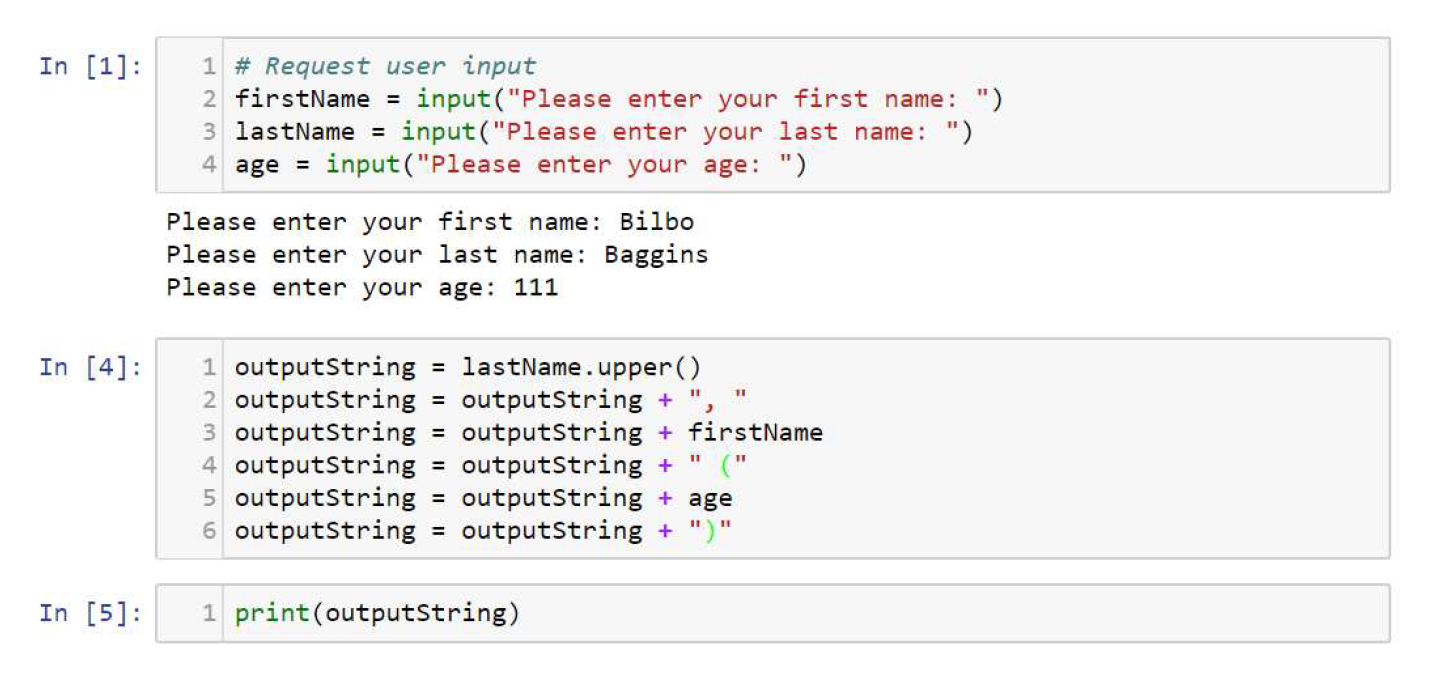
\includegraphics[width=\textwidth]{../IMG/3E03.png} 
\end{figure}


Which output is produced by the last line?
\begin{enumerate}[label=(\alph*)]
	\item {\code{Baggins, BILBO (111)}}
	\item {\code{Bilbo BAGGINS (111)}}
	\item {\code{BAGGINS, Bilbo (111)}}
	\item {\code{BAGGINS, BILBO (111)}}
	\item {\code{BILBO BAGGINS 111}}
	\item {\code{BAGGINS, Bilbo()111()}}
\end{enumerate}


\textit{Hints:
You can copy the code into Jupyter Notebook and check your understanding of the functions
is correct. Make sure you understand each individual step.}\\[1cm]


% ------------------------------------------------------------------------------


\subsubsection*{Exercise 3.E04}
Write a program that accepts an arbitrary user input and then lists the number of each
vowel (a, e, i, o, u) in the string. Your output should look something like this:\\

{\code{The string "Kermit" contains:}}\\
\hspace*{5mm}{\code{- ‘a’: 0 times}}\\
\hspace*{5mm}{\code{- ‘e’: 1 times}}\\
\hspace*{5mm}{\code{- ‘i’: 0 times}}\\
\hspace*{5mm}{\code{- ‘o’: 0 times}}\\
\hspace*{5mm}{\code{- ‘u’: 0 times}}\\


\textit{Hints:
Use the {\code{input()}} function to request user input and the {\code{print()}} function to display information. Use the {\code{count()}} operator to count the occurrences of a specific letter in the string. Remember: You can generate tabs within string using {\code{\textbackslash t}}. Depending on how you display the results you might need to convert integers into strings first using the {\code{str()}} function.}\\[1cm]


% ------------------------------------------------------------------------------


\subsubsection*{Exercise 3.E05}
Initialize a variable containing the string {\code{"Velociraptor"}}. Extract the following characters by calling their respective indices:
\begin{enumerate}[label=(\alph*)]
	\item {\code{"V"}}
	\item {\code{"l"}}
	\item {\code{"a"}}
	\item {\code{"o"}}
\end{enumerate}


\textit{Hints:
Each character in a string is assigned an index starting at 0. To extract the character
corresponding to index i from a string str use: {\code{str[i]}}.}\\[1cm]


% ------------------------------------------------------------------------------


\subsubsection*{Exercise 3.E06}
Write a program that asks the user for their first and last name (use two separate commands
for this). Then display the input in the following format:

\begin{center}
	{\code{Cookie Monster [CM]}}
\end{center}

Where the initials are added in brackets after the name.


\textit{Hints:
Use the {\code{input()}} function to request user input and the {\code{print()}} function to display information. Remember: You can extract individual characters from a string with the
following syntax: {\code{str[i]}} where i is the index corresponding to the character you want to
extract.}\\[1cm]


% ------------------------------------------------------------------------------


\subsubsection*{Exercise 3.E07}
Initialize a variable containing the string {\code{"Allosaurus"}}. Using character indices extract the
following substrings:
\begin{enumerate}[label=(\alph*)]
	\item {\code{"Allo"}}
	\item {\code{"osau"}}
	\item {\code{"urus"}}
	\item {\code{"losauru"}}
	\item {\code{"us"}}
\end{enumerate}

\textit{Hints:
Remember: You can extract substrings from a string str using the following syntax:
{\code{str[i:j]}} where i and j are indices. Note that {\code{[i:j]}} will extract characters from index {\code{i}} up to but excluding index {\code{j}}!}\\[1cm]


% ------------------------------------------------------------------------------

\newpage
\section{Difficulty: MEDIUM}

\subsubsection*{Exercise 3.M01}
Write a program that asks the user for any arbitrary input and returns the number of characters in the input string.\\
Bonus:\\
Display the number of character in the string using the following format:
\begin{center}
	{\code{You have entered the string [STRING] which contains [NUMBER] characters.}}
\end{center}
Where [STRING] is the user input and [NUMBER] the number of characters within.\\


\textit{Hints:
Use the {\code{input()}} function to request user input and the {\code{print()}} function to display information. Use the {\code{len()}} function to count the characters in a string.
For the Bonus exercise: You will need to make sure all variables are of the primitive data type
string otherwise the string concatenator will run into an error. To convert the length of the
string (which is a number) into a string use the type conversion function {\code{str()}} (see exercise 2.M06).}\\[1cm]


% ------------------------------------------------------------------------------

\subsubsection*{Exercise 3.M02}
Using the in operator, check whether:
\begin{enumerate}[label=(\alph*)]
	\item {\code{"b"}} is part of {\code{"London"}}
	\item {\code{"Z"}} is part of {\code{"Zimbabwe"}}
	\item {\code{"V"}} is part of {\code{"Denver"}}
	\item {\code{"t"}} is part of {\code{"Tokyo"}}
	\item {\code{" "}} is part of {\code{"New York"}}
	\item Request a string and a character from the user then check whether the character is
contained in the string.
\end{enumerate}


\textit{Hints:
Remember that Python is case sensitive. Use the {\code{input()}} function to request user input.}\\[1cm]




% ------------------------------------------------------------------------------

\subsubsection*{Exercise 3.M03}
Copy the following corrupted data lines into your Jupyter Notebook:
\begin{center}
	{\code{"In a hole inXXXXXXXXXXX the ground there lived a hobbit.XXXX Not a nasty,XXXXXXXXXX dirty, wet hole, filled with theXXX ends of worms andXXXXX an oozy smell, nor yet a dry, bare, sandy hole with nothing in it to sit down on or to eat: it was aXXXXXXXXXXXX hobbit-hole, and that means comfort."}}
\end{center}

Using the {\code{replace()}} function, remove all occurrences of {\code{X}} from the string and display the cleaned-up line.\\


\textit{Hints:
Removing a character all together is the same as replacing it with an empty string.}\\[1cm]


% ------------------------------------------------------------------------------

\subsubsection*{Exercise 3.M04}
Look at the following code:
\begin{figure}[H]
		\centering
		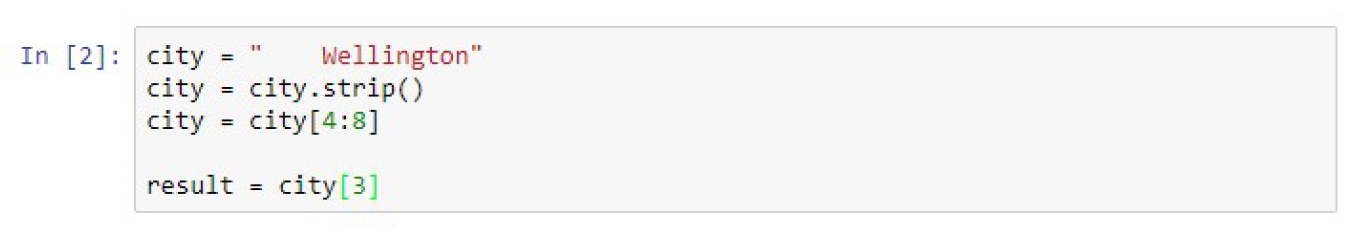
\includegraphics[width=\textwidth]{../IMG/3M04.png} 
\end{figure}
What is stored in the variable {\code{result}}?\\


\textit{Hints:
If you are unsure you can reproduce the command lines one by one in Jupyter Notebook.}\\[1cm]


% ------------------------------------------------------------------------------

\subsubsection*{Exercise 3.M05}

Ask the user to give their full name. You will obtain input strings looking like this: \begin{center}
	{\code{"Cookie Monster"}}.
\end{center}
Take the strings an extract the first letter of the first name and the first letter of the last
name and display the entire name in the following format:
\begin{center}
	{\code{Cookie Monster [CM]}}
\end{center}
Where the initials are added in brackets after the name.\\


\textit{Hints:
You can solve this individually for each dataset by counting the indices and extracting
substrings manually. However, what you want is a code that can handle all data sets of this
format. So instead consider what they all have in common: Blanks as separators.
Use the find() operator to determine the index of the blank. Then extract a substring from
the beginning of the original string to the index of the blank. This is the first name. Extract a
second substring from the index of the blank to the end of the string. This is the last name.
Extract the first letters of both first and last name and combine everything in your output.}\\[1cm]


% ------------------------------------------------------------------------------

\subsubsection*{Exercise 3.M05}
Start with the following data set:
\begin{figure}[H]
		\centering
		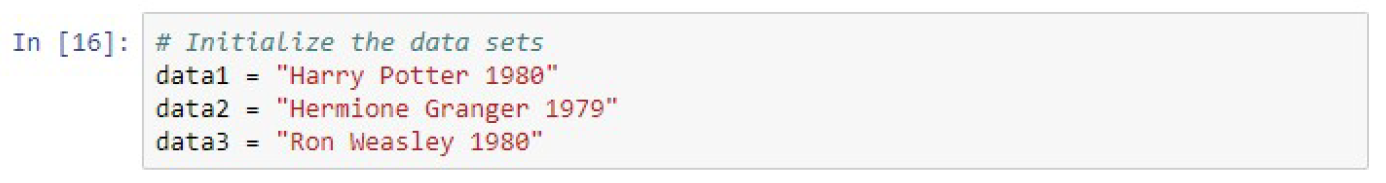
\includegraphics[width=\textwidth]{../IMG/3M06.png} 
\end{figure}
Extract the name and birth year of each person, then calculate how old they are now.
Display your results.\\


\textit{Hints:
Use the {\code{find()}} function to determine the index corresponding to the first blank. A substring from the beginning to that index will contain the first name regardless of how long it is. Take the remaining string without the first name and search again for the index of the space.
Another substring from the beginning to this index will contain the last name and the
remainder will be the year. You can then convert this final substring into a number and
calculate the age. You might also find the {\code{strip()}}, {\code{str()}} and {\code{int()}} functions useful here.}\\[1cm]



% ------------------------------------------------------------------------------

\subsubsection*{Exercise 3.S01}
Write a program that takes an arbitrary string and transforms it into a title. If a string is a
title all words start with a capital letter. For example:\\
{\code{"harry potter and the prisoner of azkaban"}} is a normal string.
{\code{"Harry Potter And The Prisoner Of Azkaban"}} is a string in title format.\\


\textit{Hints:
You could use the {\code{find()}} function, extract each word individually, transform the first letter into an upper case letter and then recombine the characters. However, this seems
complicated. Instead try Google. If you search for something like "python string title
transform" you will already get relevant results. Checking out some of them will tell you that
the function you’re looking for exists and is called title(). If you search specifically for the
python string operator {\code{title()}} you will find the following website:
\url{https://docs.python.org/2/library/stdtypes.html}. Scroll down until you find {\code{str.title()}}. The corresponding paragraph tells you how to use the function.}\\[1cm]


% ------------------------------------------------------------------------------

\subsubsection*{Exercise 3.S02}
You are given a list of student email addresses. Every email address follows the same format:
studentNumber@hogwarts.ac.uk, for example: 12345678@hogwarts.ac.uk.\\
Write a program that accepts any email address and extracts the corresponding student
number.\\


\textit{Hints:
Consider what all email addresses have in common: They all end with @hogwarts.ac.uk and
everything before that is the student number. So you want to extract a substring from the
beginning up until but excluding the @ symbol. Use the {\code{find()}} function to determine the
index of the @ symbol and then slice the string.}

% ------------------------------------------------------------------------------


\newpage
\section{Difficulty: HARD}


\subsubsection*{Exercise 3.H01}
Write a program that asks the user to give you a string and then reverses it with one command.\\

\textit{Hints:
Try to think of how you would reverse a word on a piece of paper. You would start from the
end, take down the last letter then the 2nd to last letter and so on. Translate this behaviour
into a command line.}\\[1cm]


% ------------------------------------------------------------------------------

\subsubsection*{Exercise 3.H02}
Write a code that asks the user how many animals of a specific type (cow, pig, horse, goat, dog, and cat) are on a farm. Then, using the {\code{format()}} function, display the information you have gathered in the following format
\begin{center}
	{\code{"There are 50 cows, 30 pigs, 3 horses, 3 goats, 2 dogs, and 3 cats on the farm."}}
\end{center}
using one command line only.\\


Hints:
Use the {\code{input()}} function to request user input and the {\code{print()}} function to display output.



